\renewcommand{\arcsec}{$^{\prime\prime}$} %redundant command definition, but needed for thesis template
\renewcommand{\arcmin}{$^{\prime}$}
\newcommand{\rts}[1]{{\color{violet} RTS: #1}} % RTS comment
\newcommand{\jdp}[1]{{\color{red} JDP: #1}} % JDP comment
\newcommand{\cck}[1]{{\color{brown} CCK: #1}} % CCK comment
\newcommand{\amy}[1]{{\color{cyan} ARW: #1}} 

% #1- element #2- ionization state #3 -wavelength in angstroms
\newcommand{\spetralline}[3]{#1\,{\sc #2}\,#3\,\AA}



\title{First Flight of the EUV Snapshot Imaging Spectrograph (ESIS)}

\author{Jacob D. Parker}
%\author{Roy Smart}
%\author{Charles Kankelborg}
%\author{Amy Winebarger}
%\author{Nelson Goldsworth}

\begin{abstract}
    This is the abstract.
\end{abstract} 

\section{To Do List}
	\begin{itemize}
		\item Go through and clean up spectral lines with new command so they are all the same.
	\end{itemize}



\section{Introduction}
	\begin{itemize}
        \item Instrument Heritage
            Brief summary since this is a repeat of the instrument paper.
        \item Scientific Motivation and Goals
            There is A LOT of this copied from the proposal into the instrument paper.  I think it needs to be lightly summarized here.
        \item Sections Outline
    \end{itemize}

\section{ESIS Mission}
    \begin{itemize}
        \item Brief description of the instrument, mostly pointing to the instrument paper.  Describe ESIS enough so that the data levels make sense. Need to consult the instrument paper to see what fits here. 
        \item ESIS Flight info.  Time, airtime, pointing, stability, etc.  Suggestions welcome here.
        \item Summary of Coordinated Data????
    \end{itemize}
    
	\subsection{The Experiment}
		ESIS gathers an image in each of its four detectors (channels) during every exposure.  
		Each channel is identical, with its own grating and detector. They are arrayed at $45^{\circ}$ increments about the axis of symmetry of the paraboloidal primary mirror. ESIS has 4 channels currently, but is built to accommodate up to 6 (limited by interference with the optical bench).
		
		\amy{ Would not say the channels are identical, or would say identical except that they each disperse the solar image with different angles relative to solar north.  Maybe add an image like the one from Charles talk with AIA + octagon and the four detectors with dispersion axes/solar north location marked. People won't read the instrument paper.} 
    
	\subsection{Flight Performance} \label{sec:flt}


% I don't think we need this.	
%		\begin{center}
%			\begin{table}[ht]
%				\caption{ESIS Flight Event Timeline (September 30, 2019)}
%				\label{tab:timeline}
%				\begin{tabular}{lll}\hline
%					{\bf} & {\bf Event} & {\bf Time (UTC)}\\ \hline
%					0 & Launch        &    ???? \\
%					1 & Start Dark Exposures  &  ????\\
%					2 & End Dark  Exposures  &  ????\\
%					3 & Shutter Door Open     &   ??? \\
%					4 & Fine Pointing    &    \\
%					& [Ring Laser Gyroscope (RLG) Enable] & ???\\
%					5 & Data Acquisition     &     ???\\
%					6 & Shutter door close    &   ??? \\ \hline
%				\end{tabular}
%			\end{table}
%		\end{center}
	

		\begin{figure}[ht]
			\begin{center}
				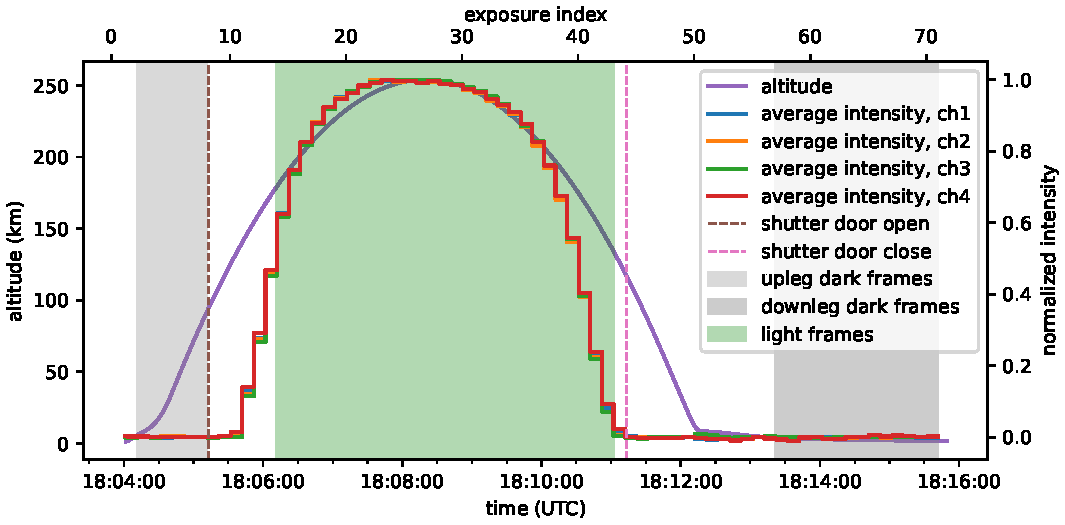
\includegraphics{figures/signal_and_altitude_vs_time}
				\caption{The altitude of the ESIS rocket determined from White Sands Missile Range radar data as a function of elapsed time from launch.  The event times listed in Table~\ref{tab:timeline} are labeled.}
				\label{fig:timeline}
			\end{center}
		\end{figure}


		ESIS was launched at 18:04:00~UTC on September 30, 2019 from White Sands Missile Range.  
		The target of observation was quiet sun at disk center.  The Solar Pointing and Aerobee Control System (SPARCS) maintained a constant target for the duration of the flight.  
		For ???\,s, ESIS recorded full detector ($\sim$2k$\times$1k) images with a 10\,s exposure and cadence. 
		Table~\ref{tab:timeline} provides the timeline of the ESIS rocket flight. Figure~\ref{fig:timeline} provides the height of the sounding rocket as a function of time, determined from White Sands Missile Range radar measurements.  The events given in Table~\ref{tab:timeline} and the approximate height at which they occurred are indicated in this figure.


	\subsection{Pointing} \label{sec:point}
		September 30th, 2019 was a very quiet day on the sun.  
		In fact, the last  B-class event detected by GOES \citep{GOES} prior to the ESIS launch was July 7th 2019 \jdp{I couldn't believe I had to go back so far so check me on this}.  
		Because of this exceptionally quiet period on the sun we chose to point at disk center, in order to minimize projection effects.  
		Despite the lack of solar activity ESIS managed to capture \jdp{do some counting} small, transient events and one significant eruption during the $\approx$5 minutes of observation.
		
		\begin{figure}[ht]
			\begin{center}
				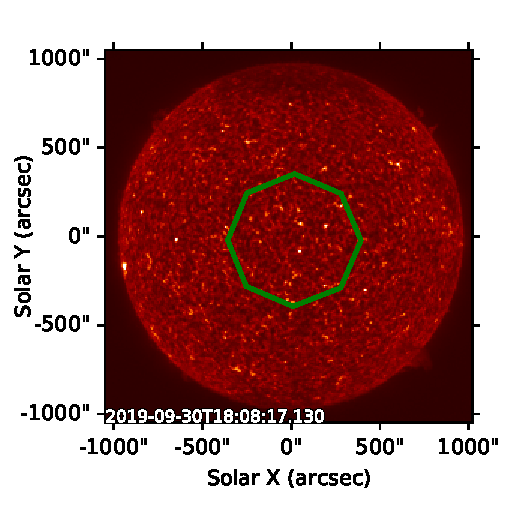
\includegraphics{esis_pointing}
				\caption{The reference AIA 304\,\AA\ data taken at 18:08:53~UT, which was used for determining the absolute pointing. The octagon indicates the ESIS FOV.}
				\label{fig:fov}
			\end{center}
		\end{figure}
	
		\begin{center}
			\begin{table}
				\caption{ESIS Flight Data Summary (*Solar coordinates; solar north at top of frame.)}
				\label{tab:data_info}
				\begin{tabular}{ll | l l}\hline
					Wavelength Range &   ???\,\AA\ \rts{max range??} & Image Size  & 2064$\times$1024\\
					Launch Date & September 30, 2019 & Field of View  & $\approx 11.3$\arcmin octagonal \rts{\fov} \\
					Data Acquisition Time & ??? - ??? \rts{\datastart--\datastop~UT} & Pointing   &  $\approx$ (15\arcsec, -35\arcsec)  \\
					Camera Gain &   [4 cameras]$2.5 \pm 0.02$\,elec DN$^{-1}$ & Roll & $??? \pm ???^\circ$ CW \\
					Camera Noise*: & & Exposure Time & 10\,s\\
					\hspace{0.2in}NE Quad \rts{Ch1} & [?,?,?,?] DN \rts{\readnoiseI} & Light Data Set: &\\
					\hspace{0.2in}NW Quad \rts{Ch2} & [?,?,?,?] DN \rts{\readnoiseII} & \hspace{0.2in}No. of Images & 29 \rts{\numdataframes (probably wrong)}\\
					\hspace{0.2in}SE Quad \rts{Ch3} & [?,?,?,?] DN \rts{\readnoiseIII} & &\\
					\hspace{0.2in}SW Quad \rts{Ch4} & [?,?,?,?] DN \rts{\readnoiseIV} & Dark Data Set & \\
					Plate Scale  & 0.??\arcsec\ pixel$^{-1}$ \rts{\platescalex, \platescaley}&  \hspace{0.2in}No. of Images & ? \rts{\numdarkframes} \\
					\hline
				\end{tabular}
			\end{table}
		\end{center}
		

		To determine the roll offset and absolute pointing post flight, the AIA\,304\,\AA\ image taken at ???~UT was used as a reference against the ESIS images taken at ???~UT.  The roll offset, found to be $\sim0.???\pm 0.005^\circ$ (clockwise about Sun center), is within the tolerances for SPARCS pointing.  Figure \ref{fig:fov} shows the full-disk AIA\,304\,\AA\ image. The ESIS FOV is indicated by the octagon.  
	
\section{Data} 

	ESIS has captured a unique data set not  available from any other source.  
	In addition, the type of data that ESIS has collected (e.g., so-called ``overlappograms'', where spatial and spectral information are overlapping) is not a data product that NASA has regularly obtained through satellite observations for many decades.  Due to the uniqueness of this dataset, we have established some data processing that different users may find useful.
	\jdp{Probably can't leave MOSES out of this Amy.} \amy{I fixed it.  Is MOSES data publicly available?  We could point to SR data sets that are overlappograms.  But now that I am thinking about it, EIS makes overlappograms when they use a slot, so maybe this isn't hte best point.  Just want to make the point that it is unique.... }
  
    We have established several levels of data processing that are described in detail below.
    Level-0 represents the raw data that was obtained by the four different cameras during flight.
    Level-1 data prepares raw CCD data for scientific work through a quadrant dependent bias and dark subtraction and gain correction. 
    Level-2 data will be corrected for atmospheric absorption and contain a header keyword tracking the correction as a function of time for use in instrument noise models.
    It will also be despiked, and contain a mask with the original data values for each corrected pixel for future respiking.
    The coefficients of a non-linear and wavelength dependent coordinate mapping from detector to solar coordinates will also be included. 
    Level-2 data is a necessary step toward inverted data products,  but will not be further described here because the results are model dependent and in development. \amy{see, I feel like you could have a 1 paragraph subsection on Level 2 that discusses some of the important parameters but doesnt' give them.  I will take a crack at it.}
    Instead, we seek a shortcut to interpretation of the ESIS data, Level-3, which allow for taking differences between images and simplified inversions.
    Level-3 data is comprised of a single spectral line cropped from Level 1 data and mapped to the sky plane via a non-linear coordinate transform.
    The highest level data product we envision providing in the future, Level 4, is the intensity as a function of $[x, y , \lambda]$, which will be the result of an inversion.
    % of the Level 2 data. \amy{Does it have to be level 2 data?  I would stop previous sentence after inversion.} 
    Since inversion is not unique, there may be multiple Level 4 products obtained by different methods.  
    Level 4 data products will be described in future publications as they become available.  
    Below each complete data level is explored in more detail.
    
    \subsection{Level 0 Data}
    		    \jdp{This likely will need to be rearranged since some of this processing goes in to prepping the Level-1 Data.}
	    Level 0 data is the raw data collected during the ESIS rocket flight.  
	    Each image is written to a fits files with on-board timestamp, camera number, and other parameters, such as the read out from temperature sensors (?) included in the header.  There were () images collected from all cameras during flight.  
	    Images taken before the shutter door opened or after the shutter door closed were used a dark images to generate Level 1 data.  
	    There were () images taken while the shutter door was open during the time of pointing stability.  
	    These images were processed into Level 1 data.  

    
    \subsection{Level 1 Data}
        \jdp{Don't forget to say something about tossing out the first two ESIS frames.}
	    \jdp{Moving Amy's comment about atmospheric absorption to this section.  Roy already has some nice plots of this and it can likely be discussed in a section explaining dark selection?}
	    
  
    
    % 	[Copied from Hi-C paper as a reminder that we need to talk about atmospheric absorption somewhere.] We use the normalized total intensities of the Level~1.0 processed flight data (processing levels described in Section~\ref{sec:data}) to assess the relative atmospheric absorption of the signal as a function of flight time.  The transmission, shown in Figure~\ref{fig:absorb} in combination with the payload altitude, is calculated as the inverse of the relative absorption (i.e., (absorption coefficient)$^{-1}$). More than 4 minutes of data were unaffected by the atmosphere.  The atmospheric absorption was compensated for in the Level~1.5 processed data set by multiplying the images by their respective absorption coefficient.  These coefficients are provided in the header of this processed set.
    	
    	
    	A summary of the flight data parameters, as described in the preceding sections, is provided below in Table~\ref{tab:data_info}. 
    	
    	
        The goal is to get a signal proportional to the number of photoelectons. 
        The result of the Level-1 process is the number of photoelectrons 
        The Level-1 dataset is a sequence of images derived from the Level-0 (raw) dataset.
        The images in this dataset have had camera-level effects such as pedestal, gain, and dark current removed.
        Also, the images in this dataset have had the 
        Camera-level effects such as pedestal, gain, dark current, and light-insensitive pixels have been removed from the images in this dataset.
        The images 
        This dataset removes camera-level effects from the Level-0 dataset such as pedestal, gain, dark current and light-insensitive pixels (such as overscan pixels).
        
        
        Also, Level-1 images have the light-insensitive pixels (such as the overscan pixels) removed 
    
        The goals of the Level-1 dataset are to remove camera-level effects (pedestal, gain, and dark current), trim light insensitive pixels, and to remove spikes. to prepare for the images for coalignment.
    
       Raw ESIS data (Figure \ref{fig:Level0}) must first be corrected for quadrant dependant gain and bias, have overscan and blank pixels removed, and be dark subtracted prior to further analysis.
       
	       \cck{Seems like you have tried to write this a few different ways. Maybe starting with a sentence about the goal (signal proportional to photoelectrons), and then presenting an enumerated list of steps. Subsequent narrative can explain any procedures that aren't obvious or straightforward.}

	\subsection{Level 2 Data}
	Level-2 data is a necessary step toward inverted data products,  but will not be further described here because the results are model dependent. \amy{will work on this}
	\jdp{If we are going to have a subsection for these other levels, we should say less about them under "Data" and just copy what is explained there to here.}

    \subsection{Level 3 Data}
 
    
    	\newcommand{\vigfit}{[0.44, 0.34, 0.38, 0.5]}
    	\newcommand{\levthreetime}{2019-09-30T18:08:51.644}
    	
    	
    	The ESIS Level-3 data product was created to provide a co-aligned, single wavelength image in each channel for quicker identification of events with non-zero LOS velocities, and easier comparison with coordinated data that doesn't require inversion. 
    	It will also allow for single wavelength inversion prior to the completion of a more complete optical distortion model and the Level-2 data product.
    	Figure \ref{fig:coalign}a shows a final Level-3 image from Camera 1 taken at \levthreetime.
    	
  		\begin{figure}[htb!]
    		\centering
    		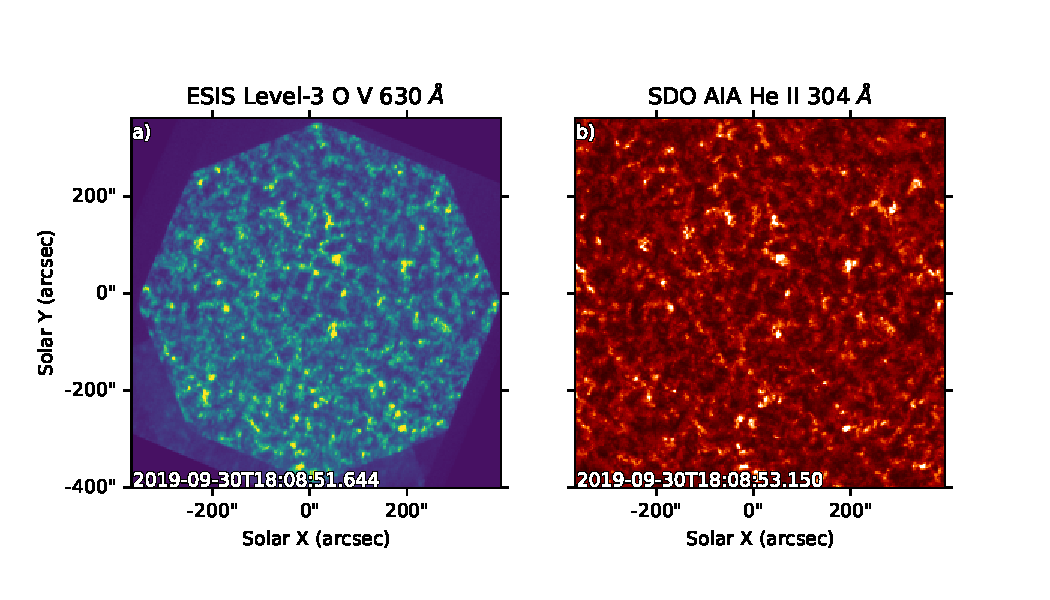
\includegraphics{aia_coalign.pdf}
    		\caption{Caption}
    		\label{fig:coalign}
    	\end{figure}
    	
    
     	In order to use Level-3 data for early inversion the intensity in DN needs to  converted to photons in order properly account for uncertainty and then normalized between channels.
   		Since each ESIS CCD has a quadrant specific gain \citep{ESIS}, the conversion from DN to photon is done to Level 1 data prior to co-alignment efforts.
   		The intensity in photons for each quadrant, $I_q$, then becomes,
   		\begin{equation}
	   		I_q = I_{DN} * G_q * 3.6\ \frac{\SI{}{\electronvolt}}{\SI{}{\elementarycharge}} * \frac{\lambda}{hc}.
   		\end{equation}
n average quadrant gain, $G_q$, of \SI[per-mode=symbol]{2.56}{\elementarycharge\per\electronvolt}, a Silicon band gap energy of \SI[per-mode=symbol]{3.6}{\electronvolt\per\elementarycharge}, and an energy per \spetralline{O}{v}{627.8} photon of \SI[per-mode=symbol]{19.6}{\electronvolt\per\photon} gives each count in $DN \approxeq 0.46$ photons.
reating Level-3 data for other wavelengths in the ESIS passband then only requires a different wavelength for conversion.
   		Normalizing the intensity of each channel is done by equalizing the image mean over a shared piece of sun, and is therefore performed after inter-channel co-alignment.
   		
   		The four ESIS channels were spatially co-aligned in two steps.  
   		First, each ESIS image is roughly cropped around the desired spectral line and then co-aligned to the closest AIA 304\,\AA\ image in time.
   		This rough cropping is why there is a remnant of the adjacent Mg {\sc x} 609.8 \AA \ spectral line in the bottom left corner of Figure \ref{fig:coalign}a.
   		AIA 304 was chosen because it is the AIA EUV channel most visually similar to O V, in both the background and bright events (Figure \ref{fig:coalign}b).
   		Prior to co-alignment each AIA image was prepped to Level-1.5 using the aiapy routines \texttt{aiapy.calibrate.update\_pointing()} and \texttt{aiapy.calibrate.register.py}  \citep{aiapy}.
   		The co-alignment was achieved through a linear coordinate transformation of the cropped ESIS image that maximizes the zero lag cross-correlation between it and AIA 304, the results of are shown in Figure \ref{fig:coalign}b.
   		Despite each image being in a different wavelength and at slightly different times we found an average zero lag cross-correlation of approximately $0.45$.
   		After the transformation each ESIS channel is re-binned to AIA resolution and can be assigned the WCS \rts{Do we have a WCS citation anywhere?}\jdp{I'll look for this.} information from AIA Level 1.5 providing pointing information and easier co-alignment with other instruments.

    	Since ESIS has a slightly non-linear distortion function \citep{ESIS}, an additional internal alignment step is performed.
    	Using a single ESIS channel as reference, in this case Camera 2, each other camera is co-aligned to it via a quadratic coordinate transformation that maximizes the zero-lag cross-correlation. 
    	After performing this additional internal alignment we find that not only is the zero-lag cross-correlation between each channel and the reference channel improved (dots in Figure \ref{fig:cc}), but also the cross correlation between every other combination of channels (stars in Figure \ref{fig:cc}).
    	Examining the cross-correlation ratio of each camera pair shows a less than 1 percent improvement in peak correlation Figure \ref{fig:cc}, demonstrating the subtle non-linearity of the ESIS optical distortion function.
    	In pixels, this corresponds to an average change in mapping of \jdp{\textbf{FIND THIS}}.
    	
     	\begin{figure}[htb!]
    		\centering
    		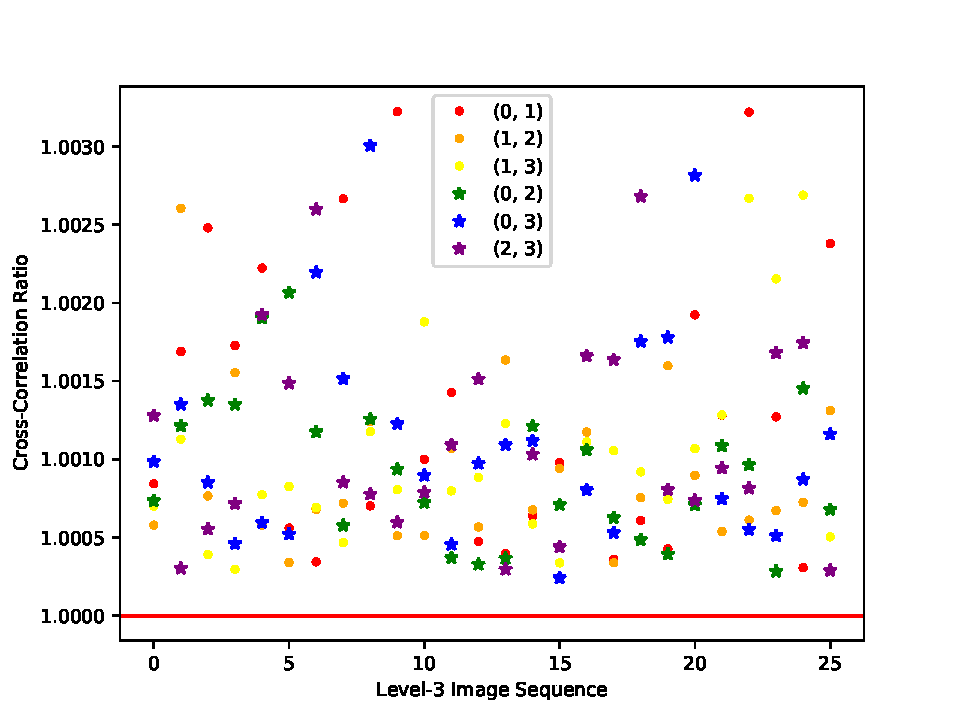
\includegraphics{internal_align.pdf}
    		\caption{For each ESIS exposure (or image sequence) every channel pair, labeled in the legend, is cross-correlated to measure internal alignment quality.  The ratio of zero lag cross-correlation after a quadratic transformation to that of a linear transformation is plotted.  Every point being above the ratio = 1 line indicates improved internal alignment for every combination of ESIS channels for each image sequence.}
    		\label{fig:cc}	
    	\end{figure}
    	
 		\begin{figure}[htb!]
			\centering
			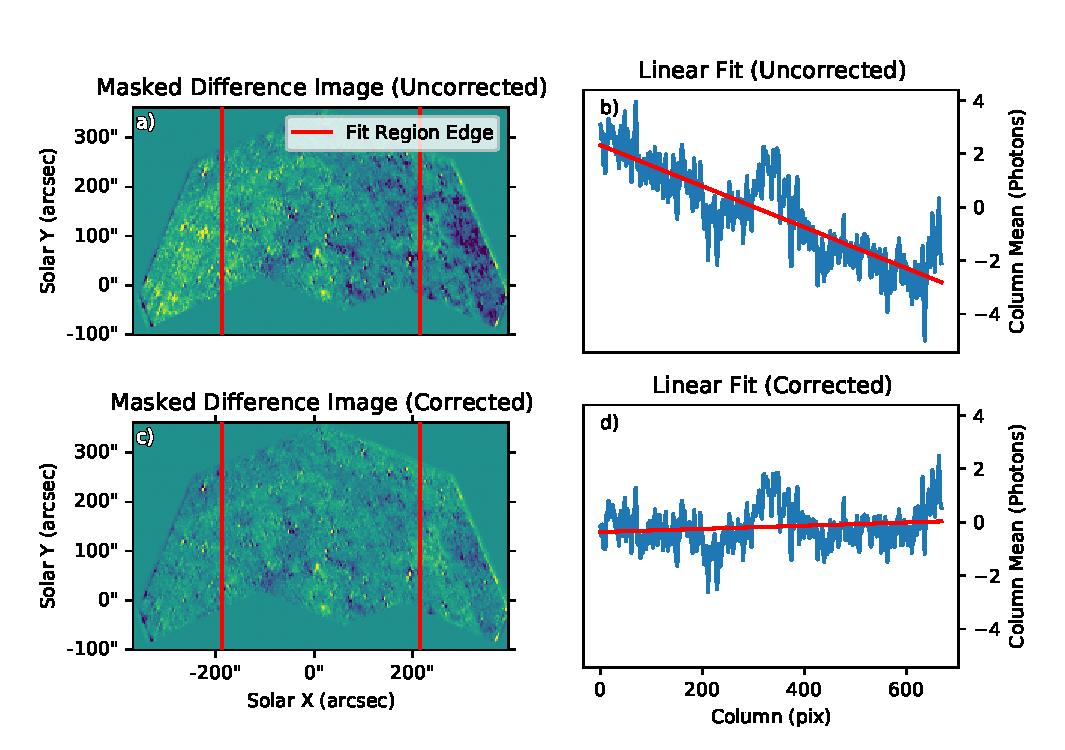
\includegraphics{vig_correct.pdf}
			\caption{Caption}
			\label{fig:vig_correct}
		\end{figure}
	       	
        Each ESIS channel has a linear trend in intensity along the dispersion direction due to internal vignetting in the optical system \citep{ESIS}.
        This linear trend in the background is very apparent in difference images that haven't been corrected (upper left of Figure \ref{fig:vig_correct}).
        To correct the trend, we divide out a linear trending background from each image with a slope oriented to the dispersion direction in each channel.
        The vignetting field divided out for each channel is,
        \begin{equation}
            V_{is} = m_{i} * (r - r_0) + 1,
            \label{eqn:vignet}
        \end{equation}
       	where,
       	\begin{equation}
       		r = x_0 + [\cos(\alpha_i)(x-x_0-x_{\text{drift}}*s) - \sin(\alpha_i)(y-y_0-y_{\text{drift}}*s)].
        	\label{eqn:vignet2}
       	\end{equation}
       	
       	In Equation \ref{eqn:vignet}, $r_0$ is equal to 65 pixels, and represents the distance from the Level-3 image edge to the ESIS field stop octagon edge at $s = 0$, the first Level-3 image sequence.
       	Also, $m_{i}$ is the slope of the vignetting field, for each channel $i$, and is a free parameter of the fit.
        In Equation \ref{eqn:vignet2},  $\alpha_i$ is the angle of rotation of each ESIS Level-3 image relative to a Level-1 image row.
        In this case, $\alpha_i = [112.5^{\circ}, 67.5^{\circ}, 22.5^{\circ}, -22.5^{\circ}]$, for cameras one through four respectively.
        The vignetting field is rotated about the origin of each image in pixels, $[x_0, y_0] = [635,635]$, to account for the change in dispersion direction.
        Because ESIS images have a pointing drift as a function of time, or image sequence $s$, the image origin is translated by $[x_{drift},y_{drift}]*s/s_t = [8_{pix},-4_{pix}]*s/26$, where $s_t $ is the total number, 28, of Level-3 images in time.
        
        \begin{figure}[htb!]
        	\centering
        	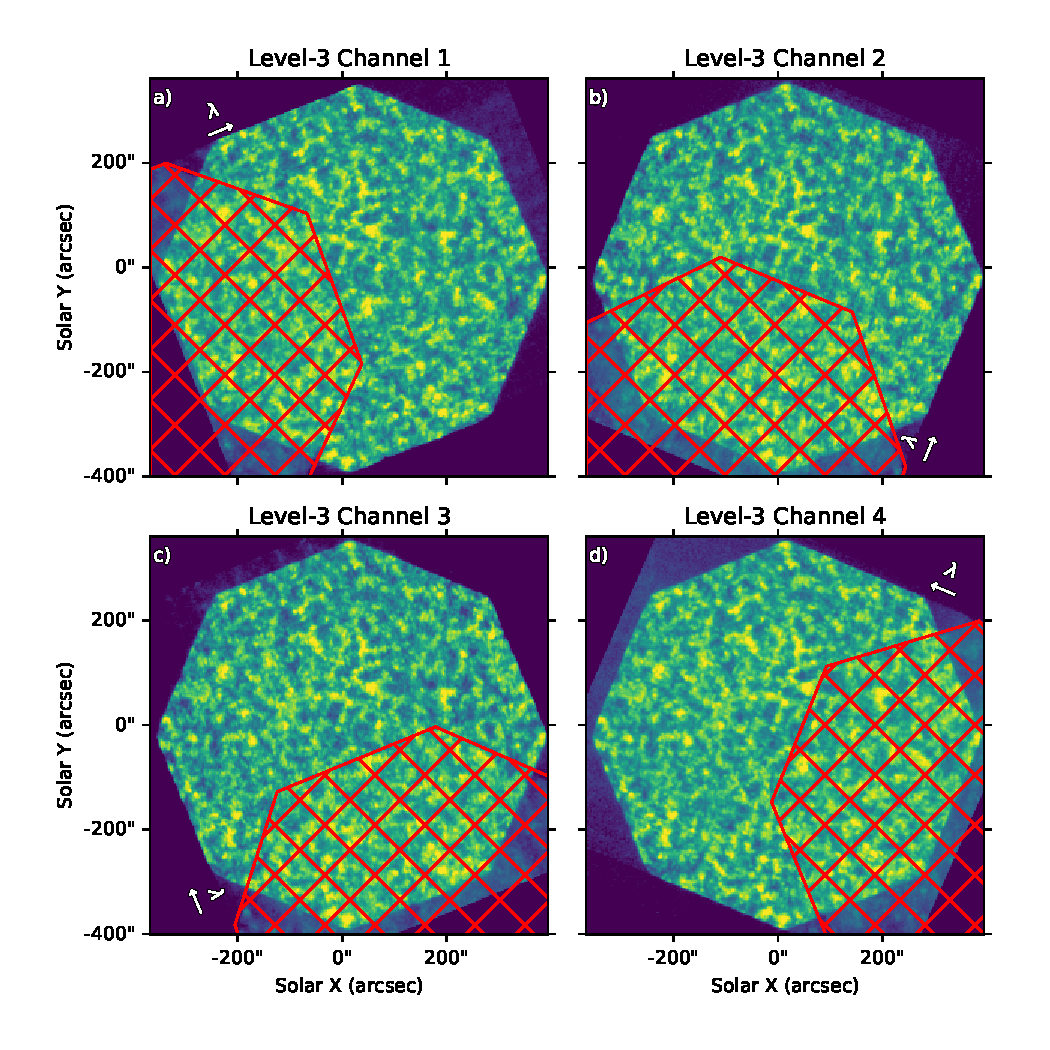
\includegraphics{mgx_overlap.pdf}
        	\caption{The red hashed region shows the overlap of the Mg {\sc x} 609.8 \AA \ spectral line in each channel that is masked prior to the vignetting correction and intensity normalization. These images are displayed in log scale in and attempt to bring out the subtle contamination.  The outline of the Mg {\sc x} can be seen very clearly in difference images like Figure \ref{fig:l3_dif}. }

        	\label{fig:mgx_overlap}
        \end{figure}
        
        When fitting for the vignetting field slope, $m_i$, for each  of the four ESIS channels we mask off the portion common to them all with no contribution from \spetralline{Mg}{x}{609.8}.
        The four channels of ESIS give 6 possible difference images for fitting the vignetting function for each image sequence $s$. 
        For each difference image we take a mean of each column and fit a line to it as a function of column position, shown in the right hand column of Figure \ref{fig:vig_correct}.
        When the average slope of all 156 fits (6 difference images per each of the 26 exposures) is minimized we consider the vignetting corrected. 
        The resulting final fit, $m_i = \vigfit$, gives smaller slopes than are predicted using ray tracing and geometric optical models \citep{ESIS}, which can be attributed to a few likely culprits.
        One source of error likely comes from the imprint of adjacent spectral lines, the most obvious being that of Mg {\sc x} 626 \AA \ visible in Figure \ref{fig:vig_correct}c.
        Since this Mg {\sc x} line overlaps almost entirely with O {\sc v}, and has an identical vignetting function, it adds intensity that prevents a perfect fit. 
        If this were the only source of discrepancy between the vignetting function predicted by the raytrace and the fits obtained from the data, then we would simply use the same, predicted vignetting for every channel. 
        However, we can anticipate slightly different vignetting in each channel due to variations in assembly so we allow each channels slope to vary independently.
        A misalignment of the ESIS field stop center, the ESIS primary optic center, and the center of the ESIS grating array, all shift the geometry of the ESIS central obscuration and can easily modify the vignetting field in each channel.
        Despite the uncertainties in vignetting, which we have found difficult to quantify, Level-3 differences are much flatter in intensity post correction as is seen in Figure \ref{fig:vig_correct}c, and will therefore lead to a higher fidelity intensity recovery when inverting Level-3 data.
        

  

\section{Preliminary Results}

	In the following subsections we will show a handful of events in the ESIS Level-3 difference images and explain how their presentation can be qualitatively interpreted as a red/blue shift or line broadening.  
	We will then demonstrate how our inversions can be qualitatively validated by these interpretations and show progress toward inverting and interpreting the largest eruption captured by ESIS.
	
    \subsection{Level-3 Difference Images}
    	Early work with MOSES images has demonstrated the utility of using differences between channels to identify solar features with significant line-of-sight velocity \citep{Fox2010,FoxPhD,RustPhD,Rust2019}, and extra spectral content \citep{RustPhD, Rust2019,Parker2021}.  
    	It is for this reason that we have chosen to develop a spatially co-aligned data product quickly that would allow us to take differences between each ESIS channel, the Level-3 data.
    	Somce each ESIS channel disperses solar features in a different direction relative to solar north, determined by the azimuthal position of each grating.
    	The positive dispersion direction in each Level-3 image is indicated with an arrow in Figure \ref{fig:mgx_overlap}.
    	Since each feature is dispersed a different direction in each channel, taking the difference between two spatially aligned channels leave only intensity away from the spectral line core.
    	For our initial analysis, we focus on the dominant O {\sc v} 629.7 \AA \ spectral line in the ESIS passband.
   		
   		\begin{figure*}[htb!]
   			\centering
   			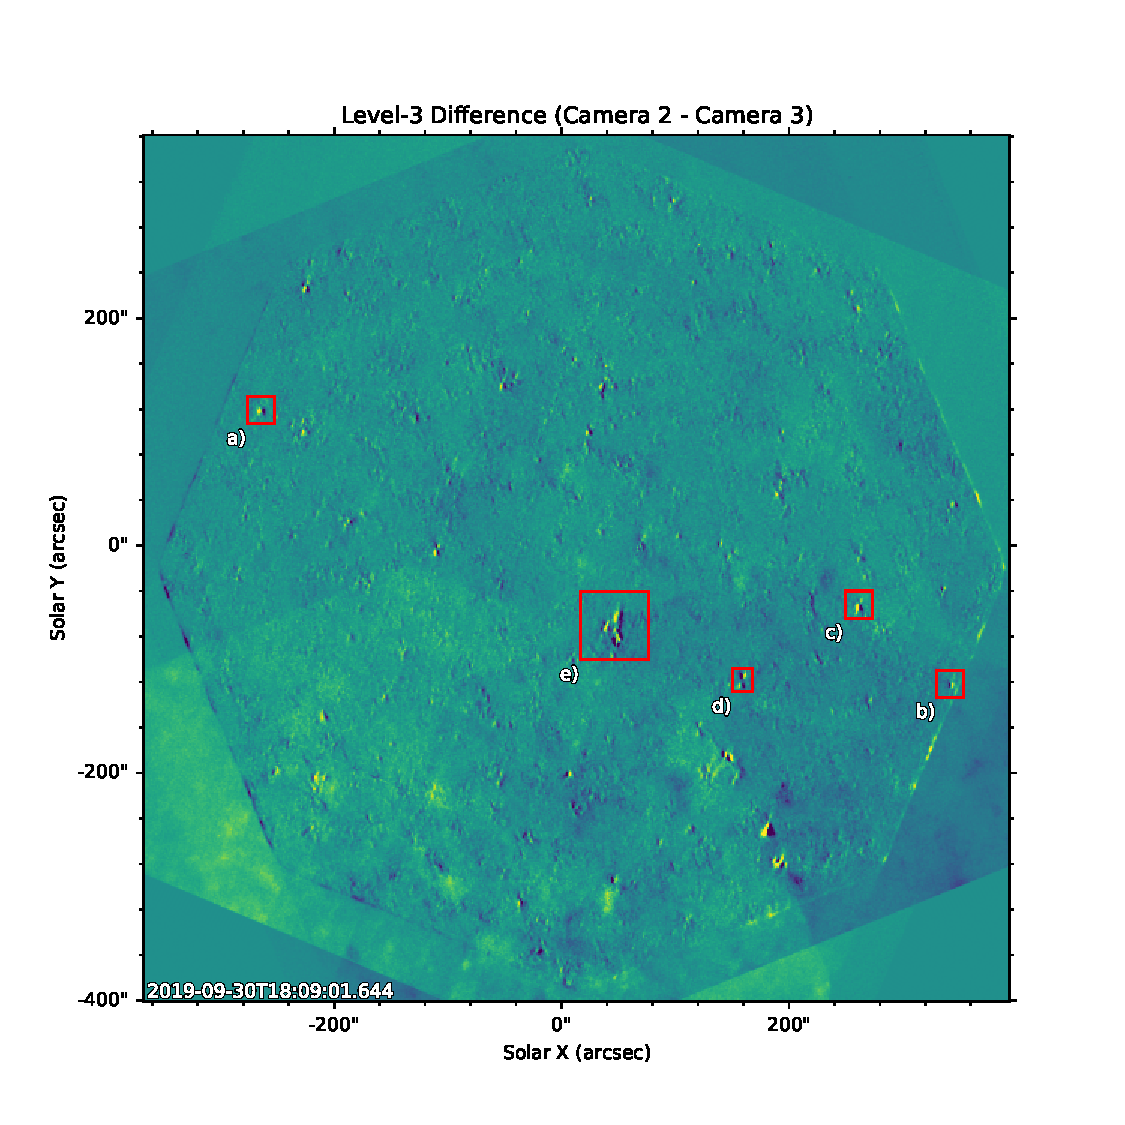
\includegraphics{l3_dif}
   			\caption{Full FOV Difference between Camera 2 and Camera 3 Level-3 images.  Events 1-3 are highlighted in Figure \ref{fig:dif_events}.}
   			\label{fig:l3_dif}
   		\end{figure*}
   	
 		\begin{figure}[htb!]
   			\centering
   			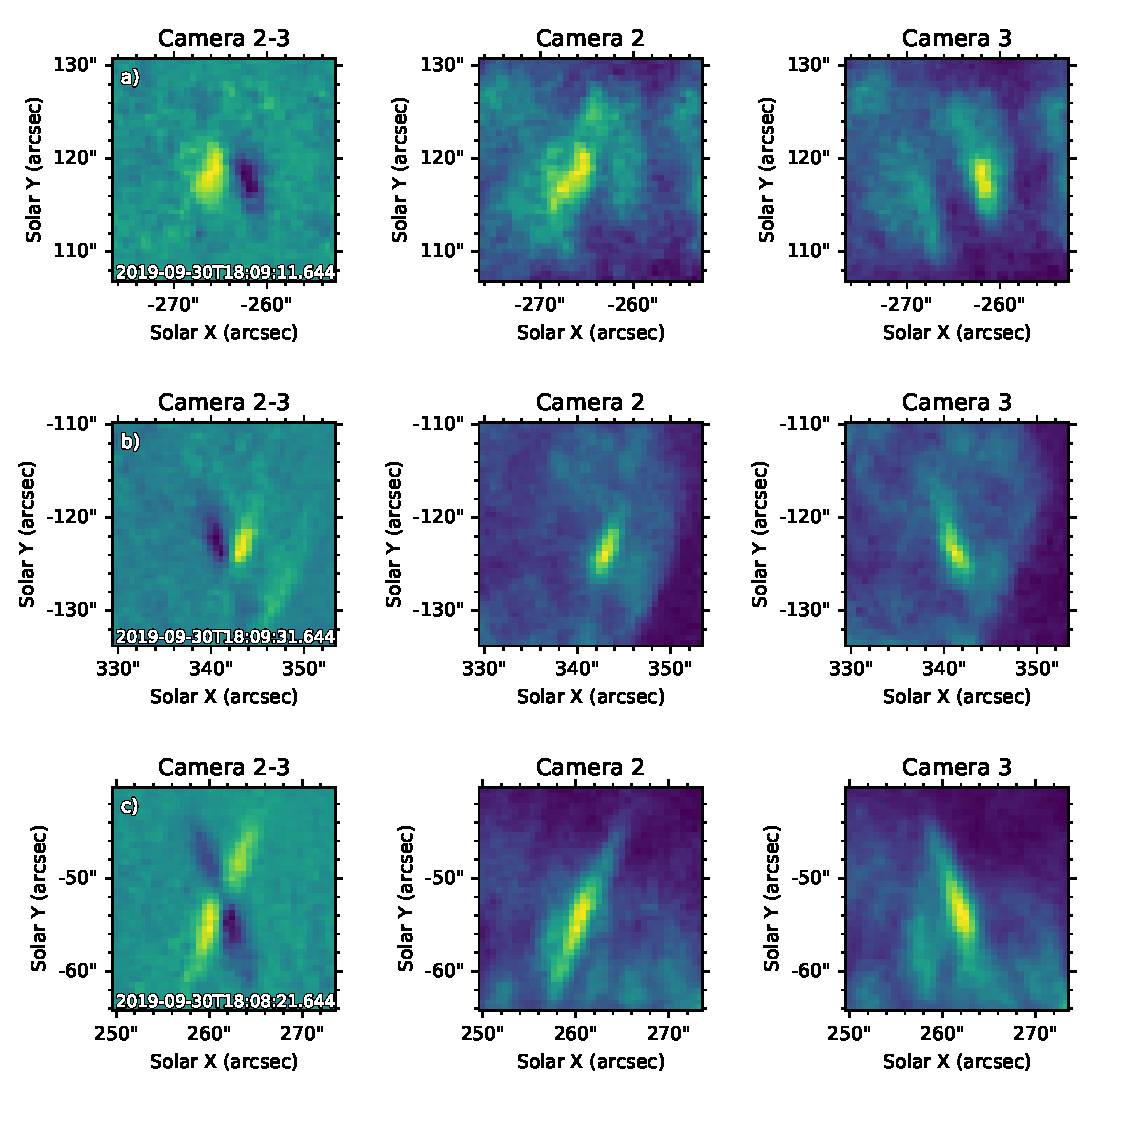
\includegraphics{dif_events}
   			\caption{Events a, b and c identified in Figure \ref{fig:l3_dif} are examples of a mostly blue, red, and broadened event respectively. The both the difference between Camera 2 and 3, and their straight intensities are included to show intensity at line center, and off.}
   			\label{fig:dif_events}. 
   		\end{figure}

    	Features in an ESIS difference image that have obvious, and nearby, positive and negative portions indicate solar events with significant LOS Doppler velocity.
    	Simple, point-like, transient brightenings with little to no spatial structure are the easiest to interpret.
    	Their naturally confined spatial extent acts similarly to a spectrographic slit.
    	Therefore, any spatial extent in an ESIS image is mostly due to spectral dispersion.
    	In these simple events, a qualitative understanding of their velocity can be ``read off'' of each ESIS image.
    	This is effect is explored in great detail by \citet{Rust2019}, who sliced through these small events along the dispersion direction and measured line profiles.
    	
    	Due to the relative orientation of each ESIS channel's dispersion axis, taking the difference of these small events leaves a V-shaped or X-shaped structure in it's place.
    	For example Figure \ref{fig:dif_events}a shows a V-shaped event that is pointed downward in the difference between the Camera 2 and Camera 3 Level-3 image.
    	Since we know that the direction of positive wavelength dispersion is up and to the right in Camera 2 and up and to the left in Camera 3 (Figure \ref{fig:mgx_overlap}) we immediately know that this event is predominantly blue shifted.
    	For opposite reasons, a upward facing V-shaped event, like in the middle panel of Figure \ref{fig:dif_events}, is predominantly red shifted.
    	X-shaped events, seen in the bottom panel of Figure \ref{fig:dif_events}, that occur equally if not more frequently than V-shaped events, indicate significant line broadening.
    	While this gives us a quick and qualitative understanding of a simple event, even the smallest amount of spatial extent in a given feature leads to an entanglement of spatial and spectral information making it very difficult to derive qualitative velocities without inversion. 
    	
    	\begin{figure}[htb!]
    		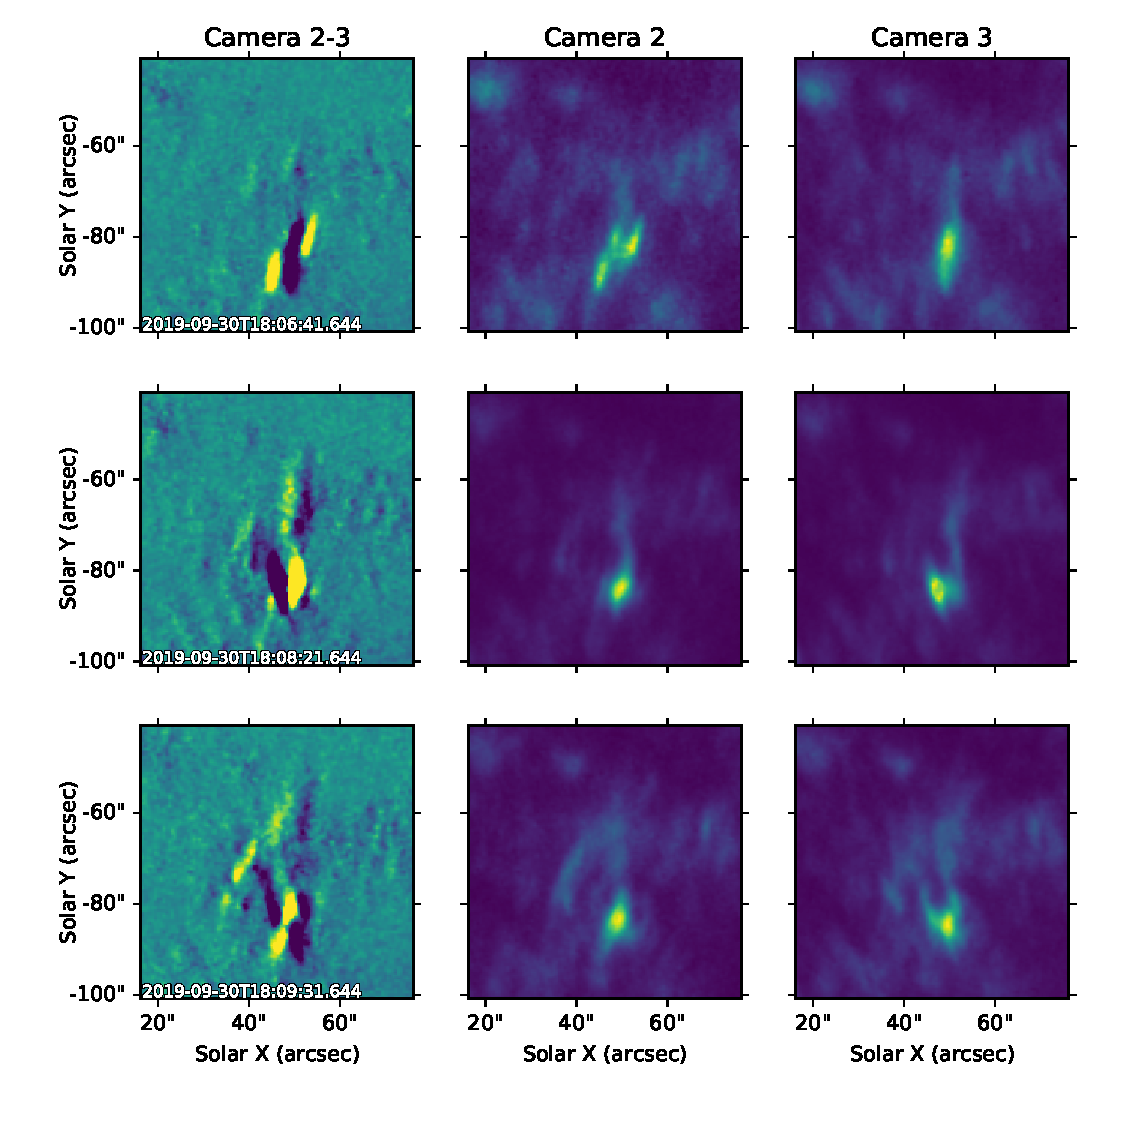
\includegraphics{main_event}
    		\centering
    		\caption{The largest eruption captured by ESIS shown at three different times. The event starts with a bidirectional flow with slight spatial separation, evolves into a strong red shift }
    		\label{fig:main_event}
    	\end{figure}
		
    	While ESIS images are littered with these simple point-like events, we also captured a handful spatially extended objects that are more difficult to interpret.
    	The most obvious of these is a much larger eruption near disk center, event d in Figure \ref{fig:l3_dif}.
    	In difference images of this event (Figure \ref{fig:main_event}) we see a mess of positive and negative features intertwined in the brightest section that sometimes present as a V or X shape, but not always, and evolve significantly in time.
    	There is also and imprint of fainter differences above the brightest knot of intensity showing motion along a spatially extended structure, likely from material being ejected from the eruption site.
    	Dynamic and spatially extended events are excellent opportunities for ESIS to shine and clearly demonstrate the need for many different projection angles (ESIS channels) if we hope to disentangle spatial information from spectra.
    	Despite the extra complexity, an understanding of ESIS difference images provides an excellent sanity check when interpreting future inversions.
    	
    
    	
    	Larger positive or negative features with no obvious counterpart nearby, are indicative of extra spectral content \citep{RustPhD,Parker2021}.
    	The most easily seen impact of this is a faint octagon edge visible in Figure \ref{fig:l3_dif} from Mg {\sc x} 625.9 \AA.
    	Extra spectral content will act as a source of error when inverting Level-3 data, but will be properly accounted for by a wavelength dependent optical distortion model and the completion of the ESIS Level-2 data set \citep{Smart2022}. 	
    
    
    
    \subsection{Early Inversions}
    	In order to better disentangle the spectral and spatial information captured by ESIS, information from every channel is combined and ``inverted'' to return a single, spatial-spectral cube, at every exposure.
    	For out preliminary inversions of ESIS Level-3 data we have chosen to use a Multiplicative Algebraic Reconstruction Technique (MART).
    	MART is attractive for our first inversions because it is fast, requires no training or assumptions about the data, and automatically enforces image  positivity.
    	We describe out particular implementation in more detail in Appendix \ref{MART}.
    	
    	
    	
    	
    	
    			
    		   	
    	
\section{Discussion/Conclusions and Future Work}





\appendix
\section{Multiplicative Algebraic Reconstruction Technique}\label{MART}
	\jdp{Now that this is floating more, I'll need to add a few things about MART and why it is attractive for this type of problem.}
	SMART adds an additional smoothing step to a simple MART applied in the past to limited-angle tomography problems like ours \citep{Okamoto1991,Verhoeven1993}.
	When testing a variety of inversion methods on MOSES data \citet{FoxPhD} identified MART as most promising of several methods in terms of speed and fidelity.
	\citet{RustPhD} applied a slightly different version of MART to the MOSES data paired with a wavelet based partial reconstruction technique for better background subtraction and event isolation.
	
	With MART we seek to reconstruct the true spatial-spectral cube, $I_{xy\lambda}$, using every ESIS image or projection, $f_{\theta x'y'}$,=. There is one ESIS image for each $\theta$ representing the relative orientations of each ESIS channel. The procedure is executed as follows:
	\begin{enumerate}
		\item \label{step:guess} Create a guess cube, $G_{xy\lambda} = 1$ on the same domain as $I$. 
		\item \label{step:contrast} Enhance the contrast of $G$ and normalize \jdp{no idea why there is an extra G + in here ...}, 
			\begin{equation}
				G \leftarrow \frac{G+G^{(1+\Psi)}}{\sum_{xy\lambda}G+G^{(1+\Psi)}}\sum_{xy\lambda}G, 
			\end{equation}
		
		\item \label{step:smooth} Convolve $G$ with smoothing kernel $K$, $G \leftarrow G * K$,
		in our case,
			\begin{equation}
			\label{eq:kernel}
				K_{ijk} = \frac{2^{3-|i|-|j|-|k|}}{64} \quad \text{for}\quad i,j,k = -1,0,1.
			\end{equation}
		
		\item \label{step:project} Sum $G_{\theta xy\lambda}$ along lines of constant $x-\delta\lambda$ to calculate a projection for each angle $\theta$,
			\begin{equation}
				f'_{\theta x'y'} = \sum_\lambda G_{\theta(x-\delta\lambda)y\lambda}, 
			\end{equation}
		where,
			\begin{equation}
				G_{\theta xy\lambda} = \mathcal{R}_\lambda(\theta)\,G_{xy\lambda},
			\end{equation} 
		and, $\mathcal{R}(\theta)$, is a rotation about the $\lambda$ axis. 	
		
		\item \label{step:chisquared} Calculate reduced chi-squared for each projection and check for convergence, in this case that $\chi_{R,\theta}^2 < 1$ , 
			\begin{equation}
				\chi_{R,\theta}^2 = \frac{1}{N_{x'} N_{y'}}\sum_{x'y'} \frac{(f_{\theta x'y'}-f'_{\theta x'y'})^2}{f'_{\theta x'y'}+\sigma^2_{RN}},
			\end{equation}
		where $\sigma^2_{RN}$ is the read noise in photons squared, $N_{x'}$ is the total number of elements along $x'$.
		
		\item Calculate correction factors for each unconverged channel, $\theta_{uc}$, weighted by $\gamma$, 
			\begin{equation} \label{eq:correctionfactor}
				c_{\theta x'y'} = \left[\frac{f'_{\theta x'y'}}{f_{\theta x'y'}}\right]^\gamma,
			\end{equation}
		where $\gamma = 2/n$ with $n$ equal to the total number of channels.
		
		\item Assign correction factors to lines of constant $x-\delta\lambda$ in the domain of $G$,
			\begin{equation}
				C_{\theta (x-\delta\lambda)y\lambda} = c_{\theta x'y'}
			\end{equation}	
		
		\item \label{step:correct} Apply a weighted product of each derotated correction to $G$ ,
			\begin{equation}\label{eq:correct}
				G \leftarrow G\left\lbrace  \,\prod_{\theta=\theta_{uc}}  \mathcal{R}_\lambda(-\theta_i)C_{\theta xy\lambda} \right\rbrace^{1/m_{uc}},
			\end{equation}
		where $m_{uc}$ is the total number of unconverged channels and 
		
		\item Repeat steps \ref{MART}\ref{step:contrast}-\ref{MART}\ref{step:correct}
		until every channel has converged at step \ref{MART}\ref{step:chisquared}.
	\end{enumerate}
		For this particular implementation we use a contrast enhancement exponent of $\Psi = .2$ and have a total number of channels, $n=4$.
		The spectral dispersion of an ESIS grating, $\delta$ is equal to 28 m\AA\ pix$^{-1}$. 
		We construct $G$ such that its resolution \jdp{bin size? step size?} in $\lambda$ is equal to $\delta$.
		All negative values introduced by rotation are set to zero after each rotation.

